% Our application is building entirely on decision making. If it seems like a \ac{pd} is coming up, buy, then sell on profit. Otherwise, wait for a \ac{pd}. Simple, yet effective if and only if the application can make accurate predictions. Our prediction algorithm needs to either detect \acp{pd} before it happens or exactly when it begins, because of the period where \ac{pd} peak span from seconds to max $10$ minutes as described in \autoref{sec:pd}. Are we too late with buying assets we may end up buying at or right before the peak which will result in a substantial loss because of the forthcoming dump. However, if we can manage to purchase assets just a few seconds in or before the \ac{pd} starts we can profit well by selling only a short time later when the coin peaks.

% For the application to have the ability to make accurate predictions, we need to carefully define a suitable algorithmic model that fits currently existing data to reverse engineer \acp{pd}. We find two paradigms \emph{financial} and \emph{\ac{ml}} as appealing fields for finding suitable algorithmic models. We encounter some problems in the field of finance, typically, financial institutions do not share their algorithms for competitive reasons, and we can not either find any models that are compatible for detecting \ac{pd} in real-time on cryptocurrency exchanges. We believe that using \ac{ml} to detect \acp{pd} is currently the optimal solution, and to reinforce that assumption, a recent PwC\footnote{Price Waterhouse Coopers is the largest network of accountants, lawyers and advisors, and deliver services within audit, consulting and tax.} study found that over the next two to three years \ac{ml} are the single most crucial technology impacting the finance function~\cite{pwc} as \ac{ml} models seem to excel financial models.


% Supervised learning problem
% binary classification problem
% Pump are anomalies
% choosing a model

% Moving on with \ac{ml}, we can define detection of \ac{pd} as a supervised \emph{binary classification} problem, \ac{pd} or not \ac{pd}. As with every supervised problem we need data that is labeled which are struggling to get.


% Our application only requires the knowledge of the pump part in a \ac{pd} to function. Our application wants to buy before or at the beginning of a pump and sell when the coin peak.

% Our application only requires the knowledge of the pump part in a \ac{pd}, as our application want to buy before or at the beginning of a pump and sell when the coin peak. We can ignore the dump part because it do not affect the decision made by our application. We can define this as a \emph{binary classification} problem, pump or not pump, or from our application perspective buy or sell.

% \acp{pd} are a common price manipulation scheme one observe on cryptocurrency exchanges, but in vast amount of existing data that exchanges produce a \ac{pd} is an \emph{anomaly}. It exist way more regular data than \ac{pd} data. This becomes problem when we want to  create a dataset containing regular data and \ac{pd} data because of the huge imbalance between the two classes, and \acp{pd} are rare entities hence it is also challenging to obtain a significant amount of \acp{pd} required to train a \ac{ml} model.

% Choosing a \ac{ml} model primarily depends on the nature of the input data. Input data can be broadly classified into sequential (e.g., voice, text, music, time series, protein sequences) or non-sequential data (e.g., images, other data)~\cite{dl_anomaly}. Cryptocurrency sources produce sequential data, more specifically \emph{time series} data. Time series data are linearly ordered sequence of values of a variable at equally spaced time intervals~\cite{stat_handbook}. 

% Anomaly detection in sequential data has attracted significant interest in the literature due to its applications in a wide range of engineering problems. \ac{lstm} neural network based algorithms for anomaly detection have been investigated and reported to produce significant performance gains over conventional methods  (Ergenet al. [2017]).

% Supervised anomaly detection techniques are superior in performance compared to unsupervised anomaly detection techniques since these techniques use labeled samples (G ̈ornitz et al. [2013]).  Supervised anomaly detection learnsthe separating boundary from a set of annotated data instances (training) and then, classify a test instance into eithernormal or anomalous classes with the learned model (testing).

% Moreover, the performance of deep supervised classifier used an anomaly detector is sub-optimal due to class imbalance (the total number of positive class instances are far more than the total number of negative class of data)~\cite{dl_anomaly}.

% Labels indicate whether a chosen data instance is normal or an outlier. Anomalies are rare entities hence it is challenging to obtain their labels~\cite{dl_anomaly}.

\chapter{Notes}

\section{Cryptocurrency}
\begin{enumerate}
    \item The market for cryptocurrencies is rapidly expanding, and at the time of writing currently had a market capitalization of around 300 billion US dollars (CoinMarketCap 2018) making it comparable to the GDP of Denmark.
    \item The lack of regulation, combined with their technical complexity, makes them an attractive target for scammers who would seek to prey on the misinformed. One such scam is know as a pump-and-dump (P\&D).
\end{enumerate}


\section{Pump-and-Dump}
\subsection{What is pump-and-dump}
\begin{enumerate}
    \item 
\end{enumerate}

\subsection{pump-and-dump scheme in context of cryptocurrency}
\begin{enumerate}
    \item In the cryptocurrency context there is an overall slightly different modus operandi than in the traditional context of penny stocks; specially, this has been seen in the rise of dedicated public \ac{pd} groups. These groups have emerged in online chat rooms such as Discord and Telegram with the sole purpose of organizing \ac{pd} scams on select cryptocurrencies\cite{P&D_to_the_moon,P&D_MIT_crypto}.
    \item price increases of up to 950\% have been witnessed, demonstrating the extent of manipulation these groups are capable of\cite{P&D_cointelegraph}.
    \item The number of members in some of the groups is reported to have been as high as 200,000 with smaller groups still running about 2000\cite{P&D_the_outline}.
    \item For these \ac{pd} groups to gain most profit, several reports of activity show that they almost exclusively target less popular coins, specially those with a low market cap and low circulation, since they are deemed easier to manipulate \cite{P&D_MIT_crypto}.
    \item There is some evidence to show that such schemes are generating millions of dollars of trading activity\cite{P&D_to_the_moon, P&D_MIT_crypto}.
    \item The Wall Street Journal published an investigative article that looked at public \ac{pd} groups and 6 months of trading activity. They found \$825 million linked to pump-and-dump schemes, with one group alone accounting for \$222 million in trades \cite{P&D_WSJ}.
\end{enumerate}

\subsection{Indicators of pump-and-dump}

Indicators of pump-and-dumps per temporal dimension and indicator type. Breakout indicators of \ac{pd}
%%% - for an analytically approach - patterns to look out for!

\subsection{Choose coins to monitor}
For these \ac{pd} groups to achieve the best results, several reports of activity show that they almost exclusively target less popular coins, specially those with low market capitalization and low circulation, since they are deemed easier to manipulate\cite{P&D_avoid_getting_duped, P&D_here_is_how, P&D_how_to_spot}. Market capitalization is defined by \cite{cryptocurrency_market_cap}. 
\begin{equation}
    C = \text{Total Current Coins} \cdot \text{Current Price}
\end{equation}
NOTE:
Missing circulation! Redefining formula
\begin{equation}
    R = \text{Volume traded for last 24 hours} \cdot \text{Current Price}
\end{equation}
Sort all market's $R$. Choose $n$ markets with smallest R.


\section{Data source selection}
% exchange selection
% Binance, Bittrex, Kraken, Kucoin, LBank.

% Cryptopia
\href{https://www.cryptopia.co.nz/}{Cryptopia} suffered a security breach January 14, 2019~\cite{cryptopia_breach_2} and was forced to shut down for a period as the breach also led to an investigation by the New Zealand Police~\cite{cryptopia_breach_1}, the law enforcement says they were acquainted with potentially unauthorized transaction activity of significant amount of cryptocurrency. Cryptopia later announced on twitter Mars 18, 2019 that they "completed their maintenance and the site is back up.", Nevertheless, we are still a bit skeptical and choose to avoid Cryptopia.

% Yobit
\href{https://yobit.net/en/}{Yobit} to all surprise on multiple occasions has announced through their official Twitter account with over 160 thousand followers~\cite{yobit_twitter}, that they are launching a coin-pump on a random coin. They even have a countdown timer on their web-page for signalizing when the coin-pump starts. In addition, various forums and articles are accusing Yobit of selling fake coins~\cite{yobit_fake_1, yobit_fake_2, yobit_fake_3}, which are most likely to be true when they have over four thousand different symbol-pairs in their Bitcoin market~\cite{yobit_market}, while there are only slightly over two thousand cryptocurrencies registered on CoinMarketCap~\cite{coinmarketcap}. We believe that Yobit has the elements of a casino where the house always wins and choosing not to play them on their own game, and collecting coin-pumps organized by Yobit may cause noise in the dataset as it necessarily do not reflect a \ac{pd}.

\begin{figure}[ht]
    \centering
    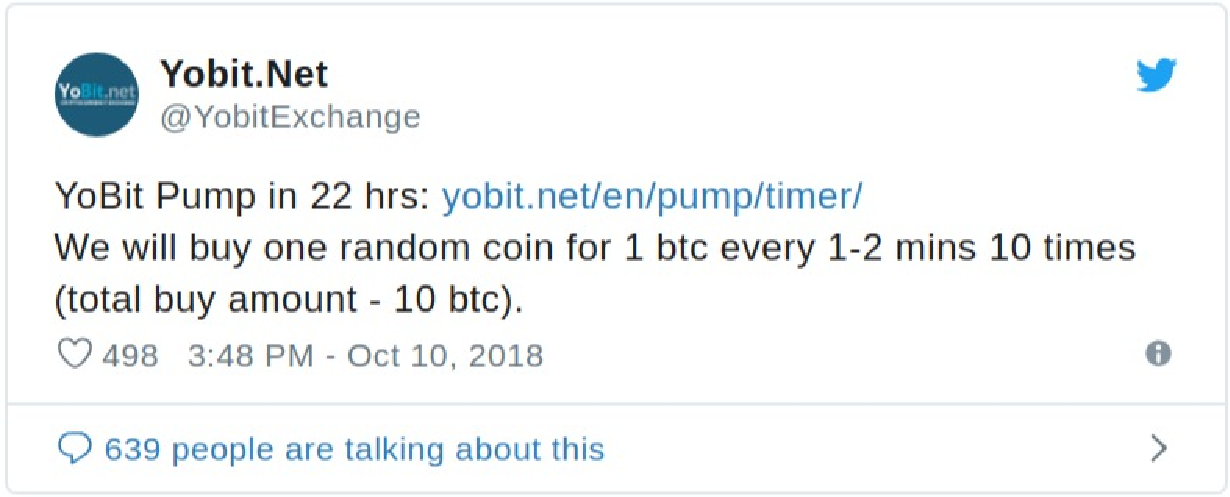
\includegraphics[width=\textwidth]{yobit.pdf}
    \caption{Yobit announcing a coin-pump through their official Twitter account}
    \label{fig:yobit}
\end{figure}

% Bittrex - banning pd

% kraken - low occurrences of pump and dump

% Binance - high volume, - lots of markets - appealing
